\section{Umsetzung der Landingpage [L]}
\label{landingpage implentation}
\setauthor{Litzlbauer Lorenz}

Der erste Entwicklungsschritt für die vollständige Single-Page-Application beginnt mit der Initialisierung der Landingpage. Aus Sicht der User-Experience war es uns wichtig, dass der*die neue Nutzer*in sofort den Verwendungszweck des Applikation begreift und dazu animiert wird, bei der Applikation mitzumachen. 

Die Entwicklung startete damit, dass die benötigten Technologien Angular, AngularThree, AngularMaterials und Bootstrap heruntergeladen wurden.

Dafür wurde der \emph{NPM} Node-Package-Manager verwendet.

\subsubsection{Angular installieren}\label{sec:AngularCLI}
Angular hat ein eigenes Tool, die Angular CLI (Command Line Interface), um Projekte zu erstellen und zu bearbeiten, sowie um Komponenten, Services und vordefinierte Codemodule hinzuzufügen.

\begin{lstlisting}[caption={{Terminalm - Angular aufsetzen, Installation der CLI, Configuration eines neuen Projektes, Starten des Projektes}},language=bash]
npm install -g @angular/cli 
ng new Gallery
? Would you like to add Angular routing? Yes
? Which stylesheet format would you like to use? SCSS   [ https://sass-lang.com/documentation/syntax#scss ]
cd Gallery
ng serve -o
\end{lstlisting}

In der ersten Codezeile wird das Angular-CLI-Tool global von NPM installiert.
Danach wird mit dem Befehl \emph{ng new} mit dem CLI-Tool ein neues Angular Projekt erstellt. Anschließend gibt es mehrere Konfigurationsauswahlmöglichkeiten. Für dieses Projekt wurde das Routing (siehe \ref{sec:Routing}) aktiviert und als Stylesheet-Formatierung SCSS ausgewählt. Daraufhin wurde in das (Projekt-) Verzeichnis Gallery gewechselt und dort mit dem Befehl \emph{ng serve} ein Webpack-Server gestartet, welcher den vorgenerierten Code von dem neu erstellen Angular-Projekt zeigt (siehe in Abbildung \ref{fig:impl:angular-starting-page}). 

\begin{figure}
    \centering
    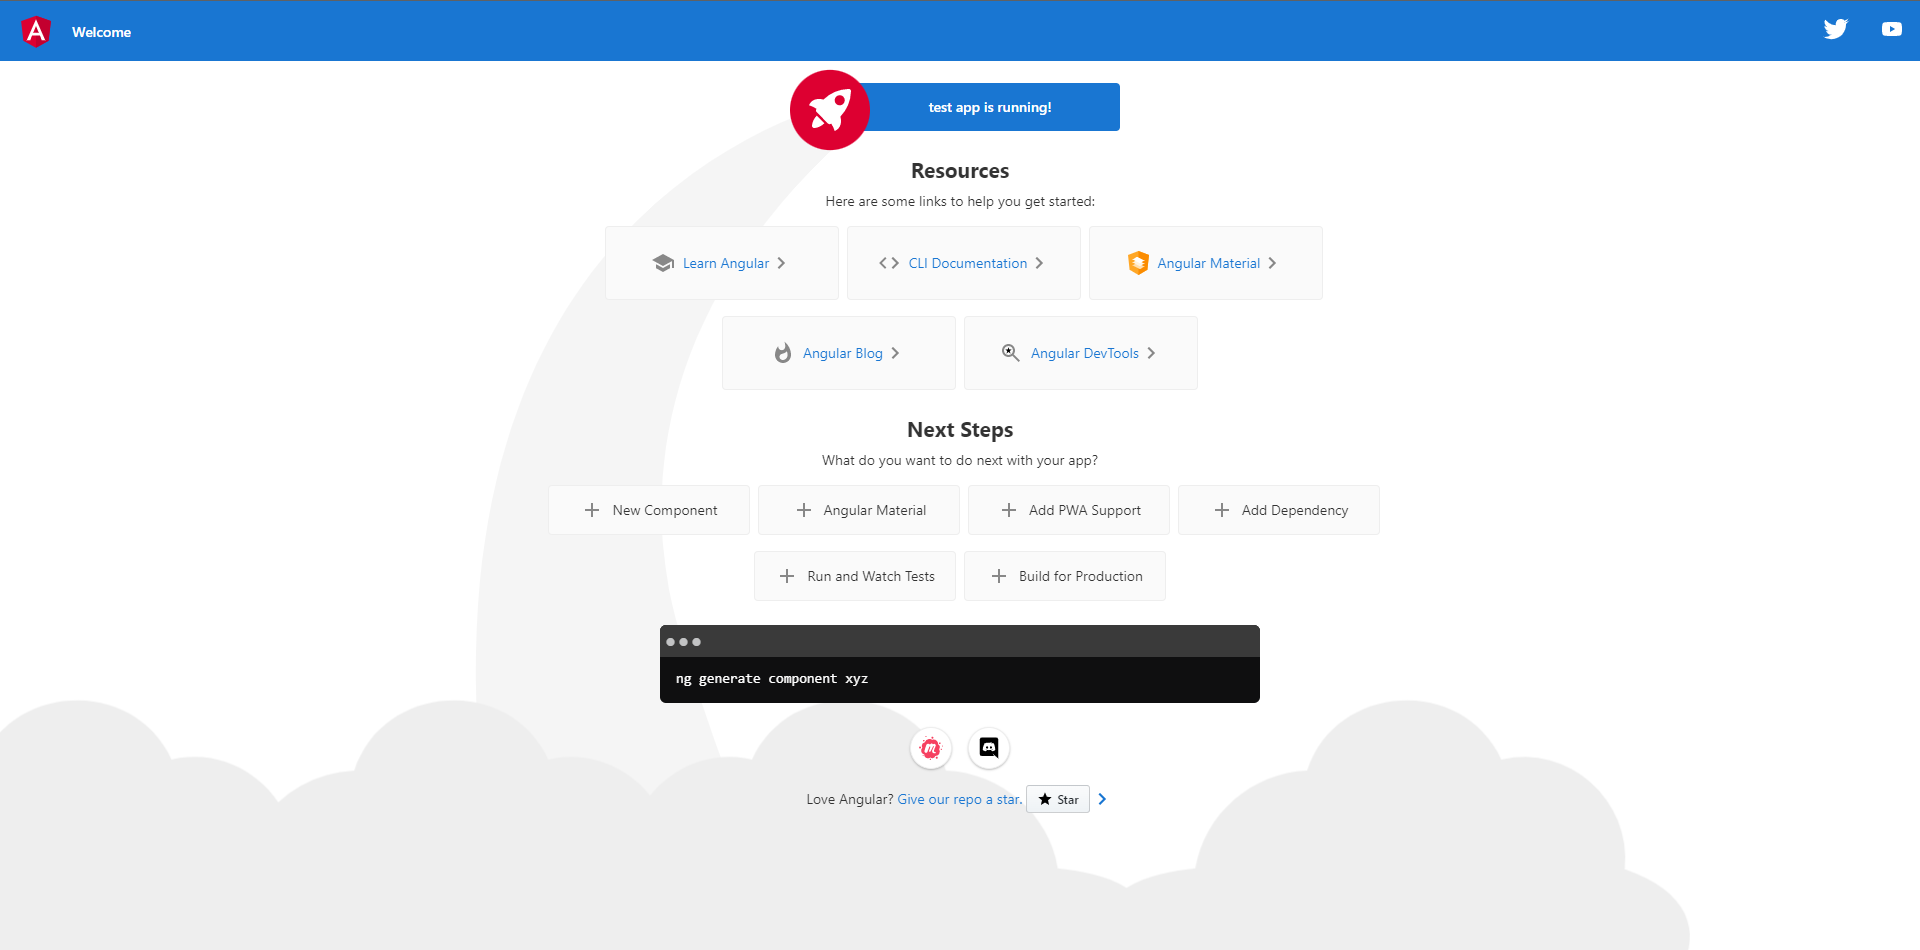
\includegraphics[scale=0.25]{pics/AngularStartingPage.png}
    \caption{Angular: Automatisch generierte Start-Webseite}
    \label{fig:impl:angular-starting-page}
\end{figure}

\paragraph{Globale oder lokale Module}
Bei einer lokalen Installation werden die installierten Module in einem Node-Modul-Computerordner lokal im Projekt abgespeichert, während alle globalen Installationen in einem einzigen Computerordner abhängig vom Computersystem gespeichert werden.

Generell kann man bei NPM-Modulen zwischen lokalen und globalen Installationen unterscheiden. Grundsätzlich wird eine lokale Installation empfohlen, referenzieren mehrere Projekte auf ein globales Modul, kann es dazu kommen, dass bei einer Aktualisierung des globalen Modules verschiedene Projekte beschädigt werden.
Das kommt daher, dass die darauf referenzierenden Projekte wegen ihrer Funktionalität anders auf die Veränderung des Modules reagieren.
CLI-Module haben eine Berechtigung dafür, global installiert zu werden. Denn CLI-Module sind abgekapselte Softwarelösungen, auf die kein anderes Projekt referenziert. Sie können auch lokal installiert werden und mit dem Befehl \emph{npx} nur im Projektordner ausgeführt werden.\cite{npmlocalorglobal}

\subsubsection{Installation der UI-Frameworks}

Nach der Installation von Angular wurden die UI-Frameworks \emph{Angular Material} und \emph{Bootstrap} installiert. 

\emph{Angular Material} konnte mithilfe des Befehls  \ref{lst:impl:installationAngularMaterials} mittels der Angular CLI in das Angularprojekt eingebunden werden.

\begin{lstlisting}[caption={{Terminal - Angular Material Installation}},language=bash,label=lst:impl:installationAngularMaterials]
    ng add @angular/material
\end{lstlisting}

Bootstrap wurde mithilfe des Befehls \ref{lst:impl:installationBootstrap} von NPM installiert.
Anschließend muss noch eine Verknüpfung zwischen Bootstrap und Angular hergestellt werden. Dafür musste in der Angular-Konfigurationsdatei \emph{angular.json} die Bootstrap Scss-Liberay eingebunden werden. Das wird in dem Code Beispiel \ref{lst:impl:BootstraptConfig} veranschaulicht.

\begin{lstlisting}[caption={{Terminal - Bootstrap Installation}},language=bash,label=lst:impl:installationBootstrap]
    npm i bootstrap
\end{lstlisting}

\begin{lstlisting}[caption={{angular.json - Bootstrap Angular Verknüpfung}},label=lst:impl:BootstraptConfig]
    {
        ...,
        "projects": {
            "Gallery": {
                ...,
                "architect": {
                    "build": {
                        ...,
                        "options": {
                            ...,
                            "styles": [
                                ...,
                                "node_modules/bootstrap/scss/bootstrap.scss"
                            ]
                        }
                    }
                }
            }
        },
        ...
    }
    
\end{lstlisting}


\subsubsection{Installation von Three.js}
Nach der Installation der UI-Libraries wurde Three.js installiert. 

\begin{lstlisting}
    npm install three
    npm i @types/three
\end{lstlisting}

\subsection{Komponenten [M]}
\label{components}
\setauthor{Fabian Maar}
Der nächste Schritt der Entwicklung ist das Erstellen der Komponenten und das Festlegen ihrer Struktur. Eine Komponente kann ebenfalls über die Angular CLI erstellt werden:

\begin{lstlisting}[caption={{Terminal - Component erstellen}},language=bash,label=lst:impl:addComponent]
    ng generate component home-page
\end{lstlisting}

\subsubsection{Allgemein}
Angular Komponenten lassen sich mit einem eigenen HTML-Selektor (z.B. <my-component>) ansprechen und in die Benutzeroberfläche einbinden. Components besitzen viele Features, die den Entwicklungsprozess, Wartung des Codes und Fehlersuche erleichtern können:

\begin{itemize}
    \item Trennung von Logik und Design
    \item Skalierbarkeit der Applikation
    \item Data-Binding
    \item Hierarchie
    \item Lesbarkeit/Übersichtlichkeit
\end{itemize}

\subsubsection{Aufbau}
Um die Logik strikt von der Benutzeroberfläche zu trennen, werden die Dateien und der Code innerhalb einer Komponente strukturiert und separiert. Eine Komponente besteht somit aus: 

\begin{itemize}
    \item einem HTML-Template, dass die Benutzeroberfläche darstellt
    \item einer TypeScript-Klasse, die die Logik und Funktionalitäten der Komponente beinhaltet
    \item einem Stylesheet, dass das Aussehen der Benutzeroberfläche beeinflusst
    \item einer TypeScript-Testklasse, um individuell Komponenten zu testen 
\end{itemize}

\cite{AngularComponentOverview}

\subsubsection{Skalierung}
Die Skalierung beschreibt, wie gut eine Applikation mit Erweiterungen und ihrem Wachstum umgeht. Dabei wird geschaut, wie leicht sich zusätzliche Änderungen und Features implementieren lassen oder wie sich die Performanz der Anwendung bei zunehmender Größe verhält. Angular unterstütz dies durch einige Features:

TypeScript hilft durch seine Code-Syntax, auch bei großen Applikationen schnell Fehler zu erkennen. 

Durch die Angular CLI kann schnell und einfach ein Grundgerüst für die Entwicklung erstellt werden. Weiteres können Components, Services und andere Angular Funktionen in jedem Entwicklungsstadium problemlos hinzugefügt werden, ohne dass der bestehende Code beeinflusst wird (siehe \ref{sec:AngularCLI}).

Angular stellt zudem Libraries wie Angular Materials oder das Component Development Kit (CDK) zur Verfügung. Dadurch können problemlos vorgefertigte Angular Komponenten und Designs zu einer Applikation hinzugefügt werden.

\cite{AngularScaling}

\subsubsection{Hierarchie}
Die Hierarchie von Angular Komponenten lässt sich wie folgt in einer Baumstruktur abbilden:

\begin{figure}
    \centering
    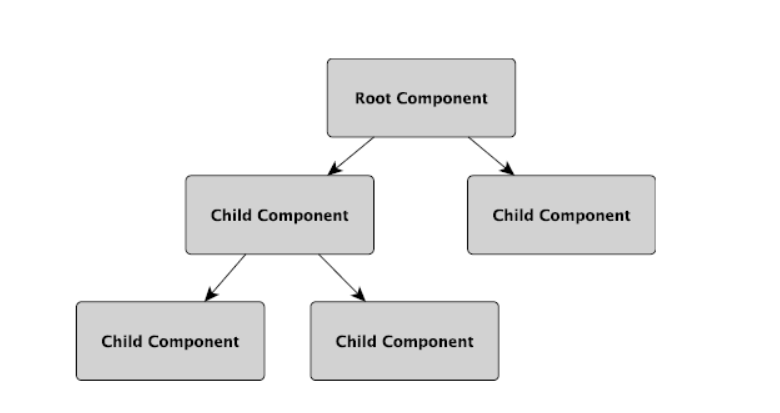
\includegraphics[scale=0.6]{pics/hierarchy.PNG}
    \caption{Component-Hierarchy \cite{AngularBuch}}
    \label{fig:tech:front:component-hierarchy}
  \end{figure}
Die Hauptkomponente ist der Root-Component. Von ihr aus lassen sich weitere Child-Components ineinander verschachteln. Diese Verschachtelung ist der Grund, warum die Anwendung in viele einzelne Teile ausgelagert werden kann. Außerdem können Komponenten durch das Data-Binding untereinander Daten austauschen.

\cite{AngularComponentsHierarche} \cite{AngularBuch}

\subsubsection{Data-Binding }
\label{data-binding}

Data-Binding ist eine Methode, Daten zwischen der Logik und der Benutzeroberfläche auszutauschen. Dabei bleibt die Website ohne Refresh immer aktuell. Das Binden von Daten kann direkt am DOM erfolgen, wofür es eine eigene Code-Syntax gibt. Beim Data-Binding wird zwischen  verschiedenen Kategorien unterschieden \cite{AngularBuch} \cite{BindingSyntax}:  
    

\paragraph{Interpolation}
Bei der Interpolation werden Daten innerhalb einer Komponente von der Datenquelle in das HTML-Template eingefügt. Die Anzeige wird auch automatisch aktualisiert, wenn sich Daten im Hintergrund ändern. \cite{BindingSyntax}

\begin{lstlisting}[caption={{Beispiel für Interpolation in der 3D-Gallery}},language=HTML,label=lst:impl:interpolation]
    <div>
    <p class="text-center py-2">{{exhibit.title}}</p>
    </div>
\end{lstlisting}

\paragraph{Property-Bindings}
Beim Property-Binding werden Daten direkt an ein DOM-Element übermittelt und ausgewertet. Somit werden die Attribute, das Aussehen und die Funktionen der jeweiligen DOM-Elemente dynamisch beeinflusst und automatisch bei Datenänderung aktualisiert. \cite{AngularPropertyBinding}
\begin{lstlisting}[caption={{Beispiel für Property-Bindings in der 3D-Gallery}},language=HTML,label=lst:impl:property-binding]
    <img [src]="user?.icon_url ?? 'assets/image/profile-photo.jpg'">
\end{lstlisting}

\paragraph{Event-Bindings}
Um auf Eingaben und Interaktionen von Benutzer*innen zu reagieren, werden Event-Bindings verwendet. Dabei werden die Daten vom HTML-Template zur TypeScript-Klasse übertragen und können dort genutzt werden. Sie sind also das Gegenstück zu den Property-Bindings. \cite{AngularEventBinding}
\begin{lstlisting}[caption={{Beispiel für Event-Bindings in der 3D-Gallery}},language=HTML,label=lst:impl:event-binding]
    <button(click)="delete()">
      <mat-icon>close</mat-icon>
    </button>
\end{lstlisting}

\paragraph{Two-Way-Bindings}
Das To-Way-Binding benutzt beide Varianten, Property- und Event-Binding, um Daten auszutauschen. Hierbei ist es möglich, die Daten sowohl von der TypeScript-Klasse zum DOM-Element zu übertragen und umgekehrt. \cite{AngularTwoWayBinding}
\begin{lstlisting}[caption={{Beispiel für Two-Way-Bindings \cite{AngularTwoWayBinding}}},language=HTML,label=lst:impl:two-way-bindings]
    <app-sizer [(size)]="fontSizePx"></app-sizer>
\end{lstlisting}
In den folgenden Kapitel werden die Komponenten und ihre Funktionalitäten näher beschrieben. 

\subsection{Routing [M]}\label{sec:Routing}
Routing ist das Konzept einer Single-Page-Applikation, wodurch die Seite niemals neu geladen werden muss und alle Daten beim Navigieren beibehalten werden können. Beim Routing werden dabei bestimmte Komponenten angezeigt, abhängig von der aktuellen URL. Dabei kann durch die Applikation navigiert werden, was durch den sogenannten Router realisiert wird.  Um das Routing überhaupt verwenden zu können, müssen die Pfade zu den zugehörigen Components initialisiert werden. Dies geschieht in einem \emph{ngModule}, wo alle initialisierten Routen über das RouterModule importiert werden. Um die Funktionalitäten und Routen für alle Components verwenden zu können, muss dieses RouterModule ebenfalls exportiert werden. Der Code zeigt dies anhand der 3D-Gallerie-Anwendung: \cite{AngularBuch}
\begin{lstlisting}[caption={Routing in der 3D-Gallery},language=TypeScript,label=lst:impl:routing]
const routes: Routes = [
  {path: '', component:HomePageComponent},
  {path: 'home', component:HomePageComponent},
  {path: 'log-signin', component:LogSigninPageComponent},
  {path: 'search', component:SearchPageComponent},
  {path: 'profile', component:ProfilePageComponent},
  {path: 'create', component:CreateExhibitionPageComponent},
  {path: 'signup', component:SignupPageComponent},
  {path: 'room/:id', component:RoomPageComponent},
  {path: '**', redirectTo: 'home'}
  ];
  @NgModule({
    declarations: [],
    imports: [ CommonModule, RouterModule.forRoot(routes) ],
    exports: [ RouterModule ]
  })

\end{lstlisting}
Hierbei steht der Pfad ‘**’ für alle ungültigen URLs wodurch der*die Benutzer*in auf die Landingpage geleitet wird.

Ebenfalls wird das Routing genutzt um das Navigieren durch die Navbar (siehe fertige Landingpage \ref{Finished Landingpage}) zu ermöglichen. Hierbei wird ein deklarierter Pfad direkt mit einem HTML-Element, über das Attribut \emph{routerLink}, verbunden. Falls sich der*die Benutzer*in auf auf dem momentanen Pfad des \emph{routerLinks} befindet, wird das Attribut \emph{routerLinkActive} aktiv. Dadurch kann dem*der Benutzer*in ein bestimmtes visuelles Feedback geliefert werden.  (siehe Code \ref{lst:impl:routerLink})

\begin{lstlisting}[caption={Routing über einen routerLink},language=HTML,label=lst:impl:routerLink]
    
          <a class="navbar-brand"
             routerLink="/home" routerLinkActive="link-activated"><mat-icon>home</mat-icon>Home</a>
          <a class="navbar-brand"
             routerLink="/search" routerLinkActive="link-activated"><mat-icon>search</mat-icon>Search</a>
          <a class="navbar-brand" *ngIf="this.auth.isLoggedIn()"
             routerLink="/profile" routerLinkActive="link-activated"><mat-icon>person</mat-icon>Profile</a>
       
\end{lstlisting}

\subsubsection{Routingparameter}
\label{Routingparameter}
Um Routen dynamisch zu deklarieren, werden sogenannte Routenparameter benötigt. Hierbei beginnt der dynamische Teil einer Route mit einem Doppelpunkt. 


\begin{lstlisting}[caption={Routingparamter in der 3D-Gallery},language=TypeScript,label=lst:impl:routingparameter]
    const routes: Routes = [
      {path: 'room/:id', component:RoomPageComponent},
      ];    
\end{lstlisting}

Um den aktuellen Zustand der URL auszulesen, muss der Router im Konstruktor injiziert werden. Anschließend kann der Parameter wie folgt ausgelesen und als Wert einer Variable zugewiesen werden:

\begin{itemize}
    \item Dies geschieht entweder über die Snapshot-Methode, die den momentanen Zustand der URL ausliest 
    \begin{lstlisting}[caption={Snapshot der URL abfragen},language=TypeScript,label=lst:impl:routingsnapshot]
        this.id = this.route.snapshot.paramMap.get('id');
    \end{lstlisting}
    \item oder, wie auch im Projekt der 3D-Gallery umgesetzt, über das Observable-Pattern auf den Router subscriben, um auf ständige Änderungen im Pfad zu reagieren:
    \begin{lstlisting}[caption={Die URL subscriben},language=TypeScript,label=lst:impl:urlsubscription]
        this.sub = this.route.params.subscribe(params => {
            this.id = +params['id'];
          })
    \end{lstlisting}
\end{itemize}
\cite{AngularBuch}